\documentclass{article}

\usepackage{fancyhdr, ragged2e, indentfirst, longtable, tabu, graphicx, float, hhline, makecell, bookmark, amssymb, multirow, array}
\usepackage[table]{xcolor}
\usepackage[letterpaper, total={7in, 9in}]{geometry}
\usepackage[export]{adjustbox}
\usepackage[tableposition=below]{caption}

\graphicspath{ {../../imgs/} }

\makeatletter
\title{Documento de Arquitectura del Software} \let\Title\@title
\date{Septiembre 2018} \let\Date\@date
\author{Ricardo Münch} \let\Author\@author
\makeatother

\pagestyle{fancy}
\fancyhf{}
\rhead{Versión: 1.0 \\ \Date}
\lhead{eFuel \\ DAS \\ Identificador del documento}

\lfoot{Confidencial}
\cfoot{iKels Consulting \\ \Date}
\rfoot{Pag. \thepage}

\renewcommand{\headrulewidth}{1pt}
\renewcommand{\footrulewidth}{1pt}
\renewcommand{\contentsname}{Índice}

\newcommand\Tstrut{\rule{0pt}{2.6ex}}       % "top" strut
\newcommand\Bstrut{\rule[-0.9ex]{0pt}{0pt}} % "bottom" strut
\newcommand{\TBstrut}{\Tstrut\Bstrut}       % top&bottom struts

\renewcommand{\cellalign}{cl}
\renewcommand\cellgape{\gape[t]}

\renewcommand{\listfigurename}{Lista de diagramas}
\renewcommand{\figurename}{Fig.}

\renewcommand{\listtablename}{Lista de tablas}
\renewcommand{\tablename}{Tabla}

\begin{document}

    \newgeometry{textwidth=12cm,textheight=10cm}
    \begin{titlepage}
        \huge{\Title}
        \begin{flushright}
            \Large{eFuel \\ Versión: 1.0}
        \end{flushright}
    \end{titlepage}

    \restoregeometry

    \newpage
    \tableofcontents

    \newpage
    \listoffigures
    \begingroup
    \let\clearpage\relax
    \listoftables
    \endgroup


    \newpage
    \begin{center}
        \begin{tabular}{ |c|c|c|c| }
            \hline
            \rowcolor{gray!30}
            Fecha & Versión & Descripción & Autores \\ [0.5ex]
            \hline\hline
            29/09/2018 & 1.0 & Documento de Arquitectura & Ricardo Münch \\
            \hline
        \end{tabular}
    \end{center}

    \newpage
    \section{Introducción}
    El objetivo principal de la arquitectura del software es aportar conceptos y un lenguaje común que ayuden a describir el software y permita la comunicación entre el cliente y los diseñadores.

    \subsection{Propósito}
    Este documento busca hacer una abstracción de lo que será el sistema a través de algunas vistas de la arquitectura del mismo. Se pretende definir algunos elementos estructurales que describen el sistema \emph{eFuel}.

    \subsection{Alcance}
    A continuación presentamos una abstracción de la estructura tiene el sistema. El documento está basado en el modelo 4+1 de arquitectura de Phillipe Kruchten. Contempla la Vista de Casos de Uso, la Vista Lógica, la Vista de Implantación, la Vista de Implementación y la Vista de Datos.

    \subsection{Referencias}
    No hace referencia a ningún otro documento.

    \subsection{Vista Global}
    Este documento comprende 6 secciones en las cuales se elaboran los distintos aspectos de la arquitectura de \emph{eFuel}, tanto a nivel de software como de hardware. En la sección \ref{reprArq} se introduce la representación arquitectónica del sistema. Seguidamente, se describen las distintas vistas que conforman la arquitectura de la sección \ref{vistaCasosDeUso} a la \ref{vistaDatos}.


    \section{Representación Arquitectónica} \label{reprArq}
    La representación arquitectónica de \emph{eFuel} está basada en el modelo de 4+1 vistas de Philippe Kruchten. En el transcurso del documento se tratarán más a fondo los detalles de cada una.

        \section{Vista de Casos de Uso} \label{vistaCasosDeUso}
    En esta vista se describirá el sistema desde el punto de vista de los casos de uso. El sistema tiene 3 actores:

    \begin{itemize}
        \item \emph{Customer}: representa a una o varias estaciones de servicio. Solo tiene acceso a la información referente a las estaciones de servicio asignadas por el administrador del sistema. Es el tipo de usuario que más uso le dará al sistema.
        \item \emph{Staff}: representa a un distribuidor de combustible. Tiene acceso a la información de todas las estaciones de servicio del sistema.
        \item \emph{Admin}: administrador del sistema. Tiene acceso al \emph{back end} de Umbraco y puede gestionar (realizar las acciones CRUD) todas las entidades del sistema, incluyendo a los usuarios.
    \end{itemize}

    \subsection{Resumen de Casos de Uso}
    \newcounter{magicrownumbers}
    \newcommand\rownumber{\stepcounter{magicrownumbers}\arabic{magicrownumbers}}
    \begin{center}
        \begin{longtable}{ | l | l | c | }
            \hline
            \rowcolor{gray!30}
            \multicolumn{1}{|c|}{ID del Caso de Uso} &
            \multicolumn{1}{|c|}{Caso de Uso} &
            \multicolumn{1}{|c|}{Actor} \\
            \hhline{===}
            \endhead

            \endfoot

            CU-\rownumber & Gestionar usuarios & Admin \\ \hline
            CU-\rownumber & Consultar lista de usuarios & Admin \\ \hline
            CU-\rownumber & Gestionar usuario (CRUD) & Admin \\ \hline
            CU-\rownumber & Asignar cliente/s a usuario & Admin \\ \hline
            CU-\rownumber & Remover cliente/s de usuario & Admin \\ \hline
            CU-\rownumber & Cambiar permisos de usuario & Admin \\ \hline

            CU-\rownumber & Gestionar contenido & Admin \\ \hline
            CU-\rownumber & Consultar lista de clientes & Admin \\ \hline
            CU-\rownumber & Gestionar cliente (CRUD) & Admin \\ \hline
            CU-\rownumber & Consultar lista de productos & Admin \\ \hline
            CU-\rownumber & Gestionar producto (CRUD) & Admin \\ \hline
            CU-\rownumber & Consultar lista de transportes & Admin \\ \hline
            CU-\rownumber & Gestionar transportes (CRUD) & Admin \\ \hline
            CU-\rownumber & Consultar lista de zonas & Admin \\ \hline
            CU-\rownumber & Gestionar zonas (CRUD) & Admin \\ \hline

            CU-\rownumber & Gestionar transacciones & Admin \\ \hline
            CU-\rownumber & Consultar lista de registros & Admin \\ \hline
            CU-\rownumber & Gestionar registro (CRUD) & Admin \\ \hline
            CU-\rownumber & Consultar lista de pedidos & Admin \\ \hline
            CU-\rownumber & Gestionar pedido (CRUD) & Admin \\ \hline
            CU-\rownumber & Consultar lista de detalles de pedidos & Admin \\ \hline
            CU-\rownumber & Gestionar detalle de pedido (CRUD) & Admin \\ \hline
            CU-\rownumber & Consultar lista de facturas & Admin \\ \hline
            CU-\rownumber & Gestionar factura (CRUD) & Admin \\ \hline
            CU-\rownumber & Consultar lista de cobros & Admin \\ \hline
            CU-\rownumber & Gestionar cobro (CRUD) & Admin \\ \hline
            CU-\rownumber & Consultar lista de detalles de cobros & Admin \\ \hline
            CU-\rownumber & Gestionar detalle de cobro (CRUD) & Admin \\ \hline

            CU-\rownumber & Iniciar sesión & Customer, Staff \\ \hline
            CU-\rownumber & Consultar lista de pedidos & Customer, Staff \\ \hline
            CU-\rownumber & Consultar pedido & Customer, Staff \\ \hline
            CU-\rownumber & Filtrar lista de pedidos & Customer, Staff \\ \hline
            CU-\rownumber & Exportar lista de pedidos & Customer, Staff \\ \hline
            CU-\rownumber & Crear pedido & Customer, Staff \\ \hline
            CU-\rownumber & Seleccionar cliente & Customer, Staff \\ \hline
            CU-\rownumber & Seleccionar fecha & Customer, Staff \\ \hline
            CU-\rownumber & Seleccionar turno  & Customer, Staff \\ \hline
            CU-\rownumber & Seleccionar transporte  & Customer, Staff \\ \hline
            CU-\rownumber & Seleccionar productos & Customer, Staff \\ \hline

            CU-\rownumber & Consultar lista de facturas & Customer, Staff \\ \hline

            CU-\rownumber & Consultar lista de clientes & Customer, Staff \\ \hline
            CU-\rownumber & Consultar cliente & Customer, Staff \\ \hline
            CU-\rownumber & Consultar pedidos de cliente & Customer, Staff \\ \hline

            CU-\rownumber & Consultar lista de transportes & Customer, Staff \\ \hline

            CU-\rownumber & Importar lista de transportes & Customer, Staff \\ \hline

            CU-\rownumber & Consultar lista de zonas & Customer, Staff \\ \hline

            CU-\rownumber & Importar lista de zonas & Customer, Staff \\ \hline

        \end{longtable}
    \end{center}

    \subsection{Diagrama de Casos de Uso}
    Se separaron los casos de uso en varios diagramas para facilitar la lectura.

    \begin{figure}[H]
        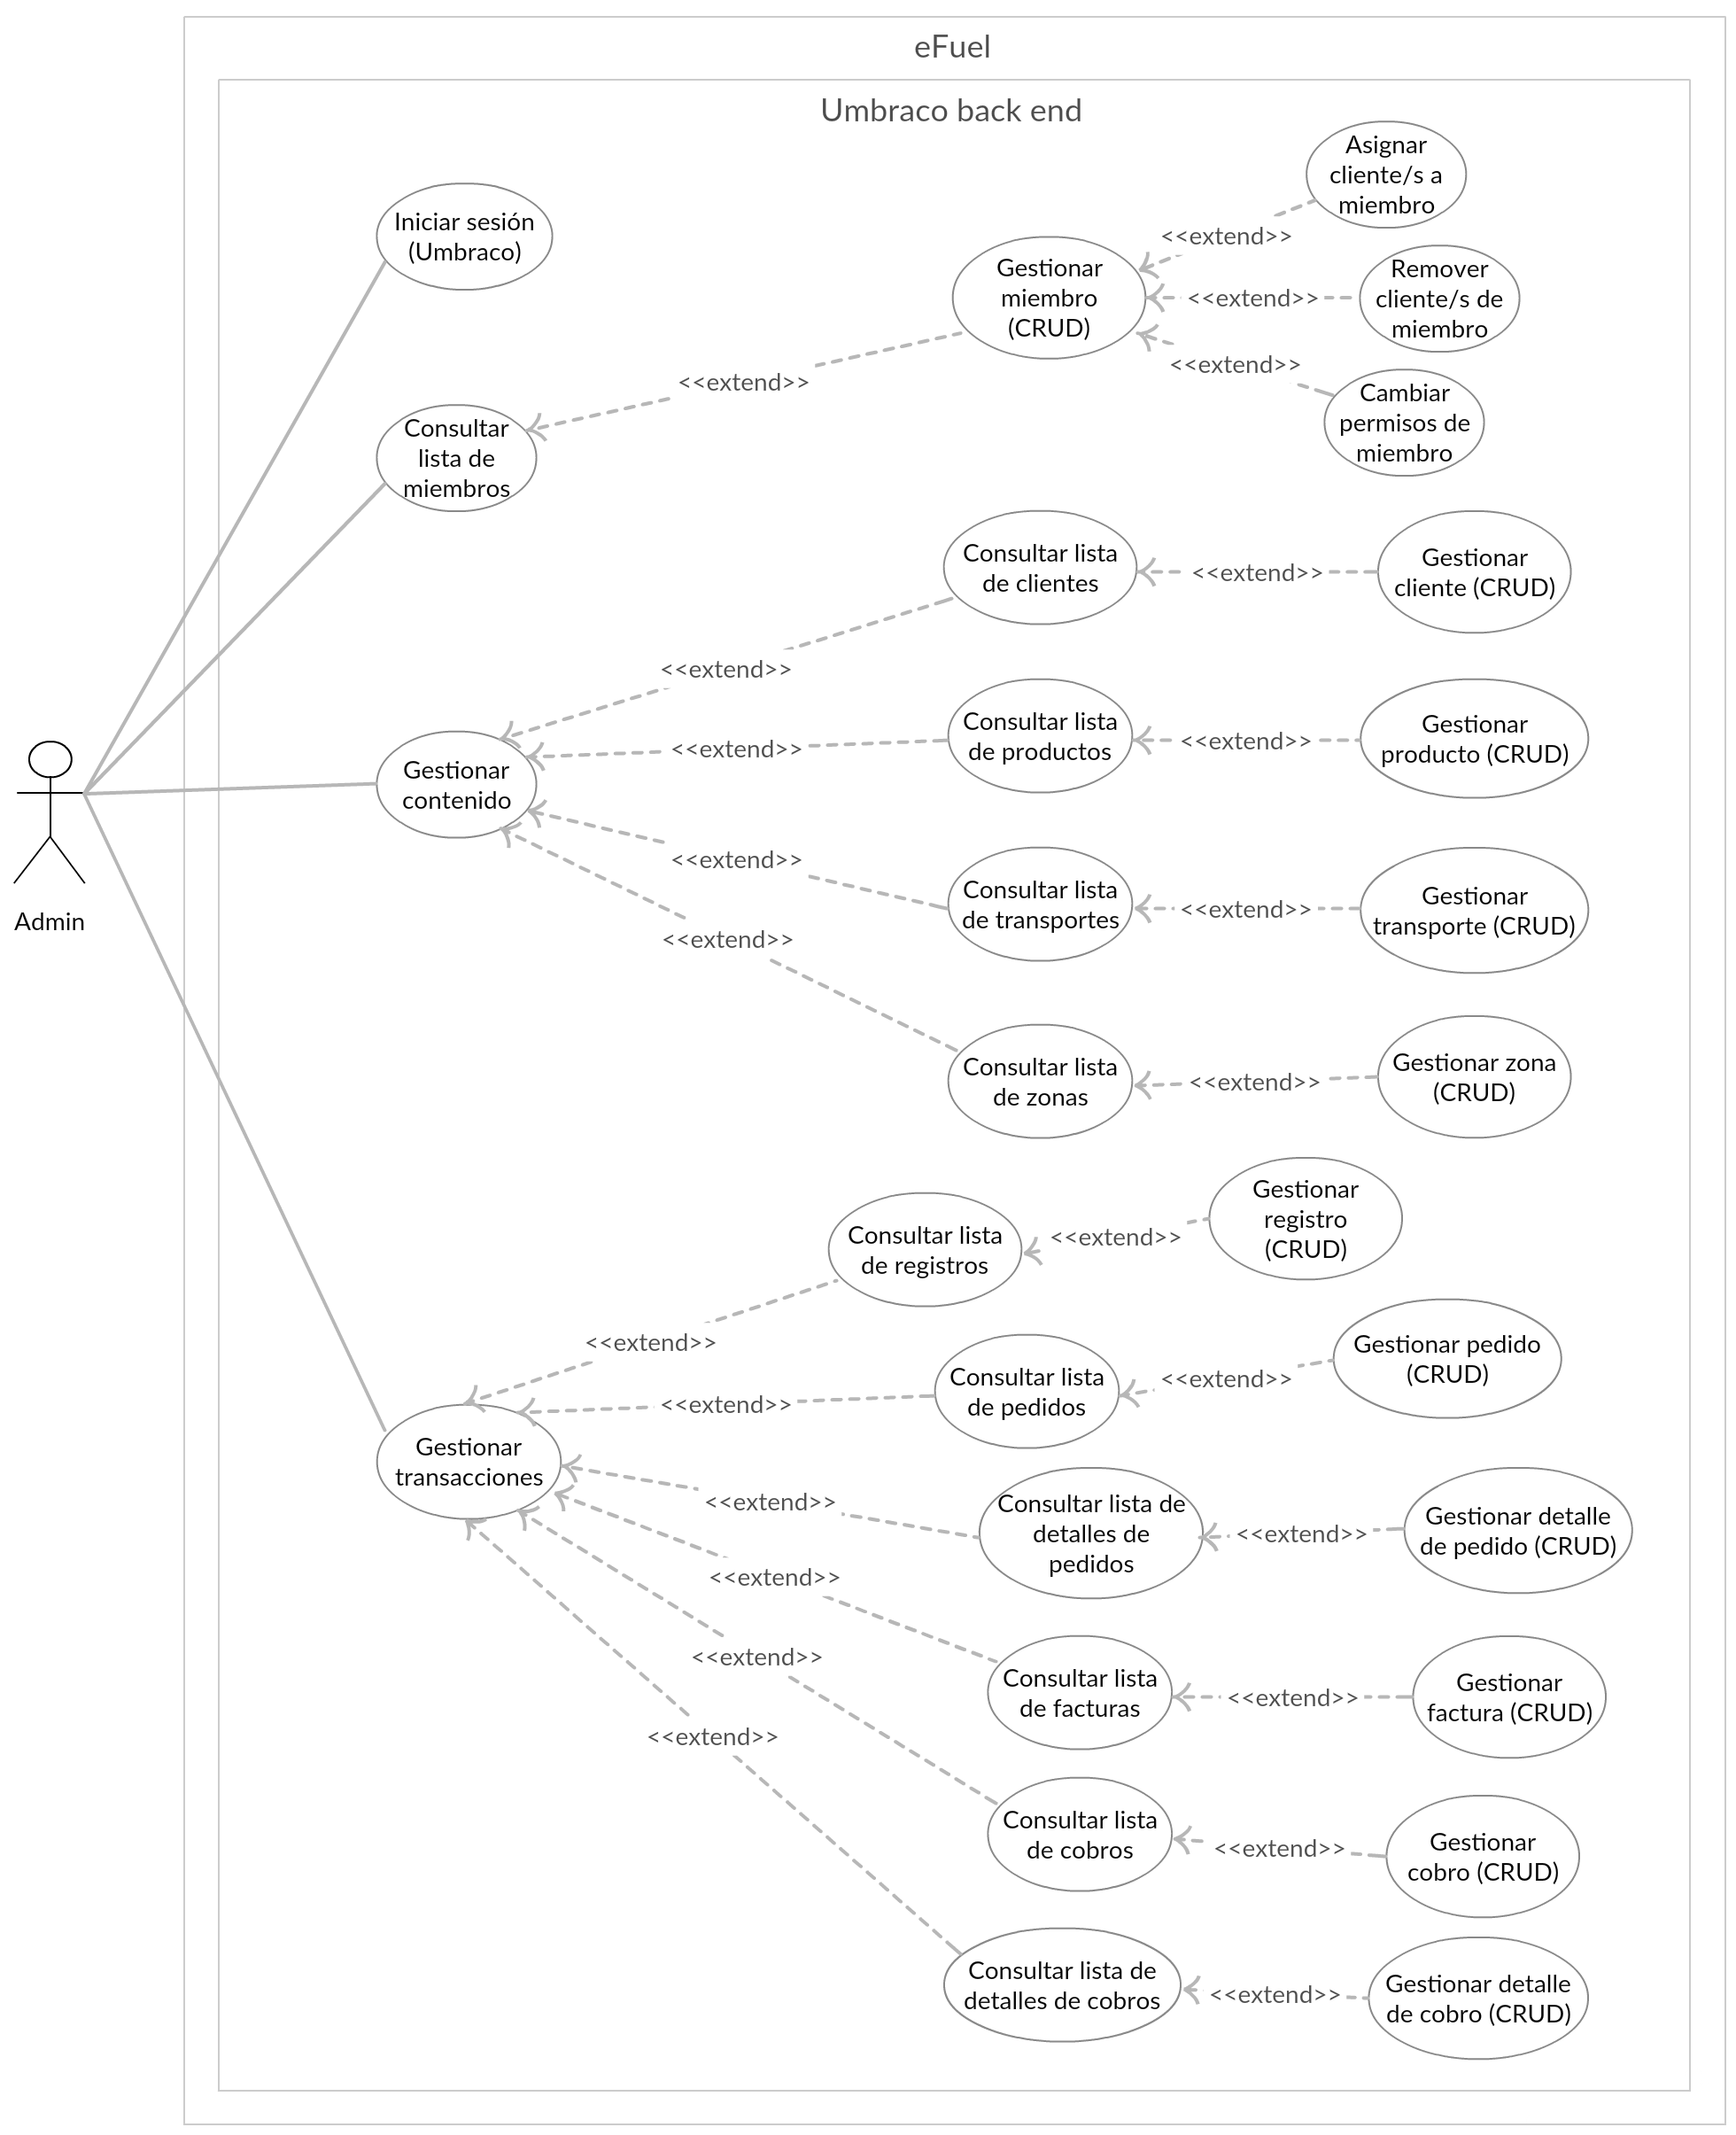
\includegraphics[width=\textwidth]{cu_admin.png}
        \centering
    \end{figure}

    \begin{figure}[H]
        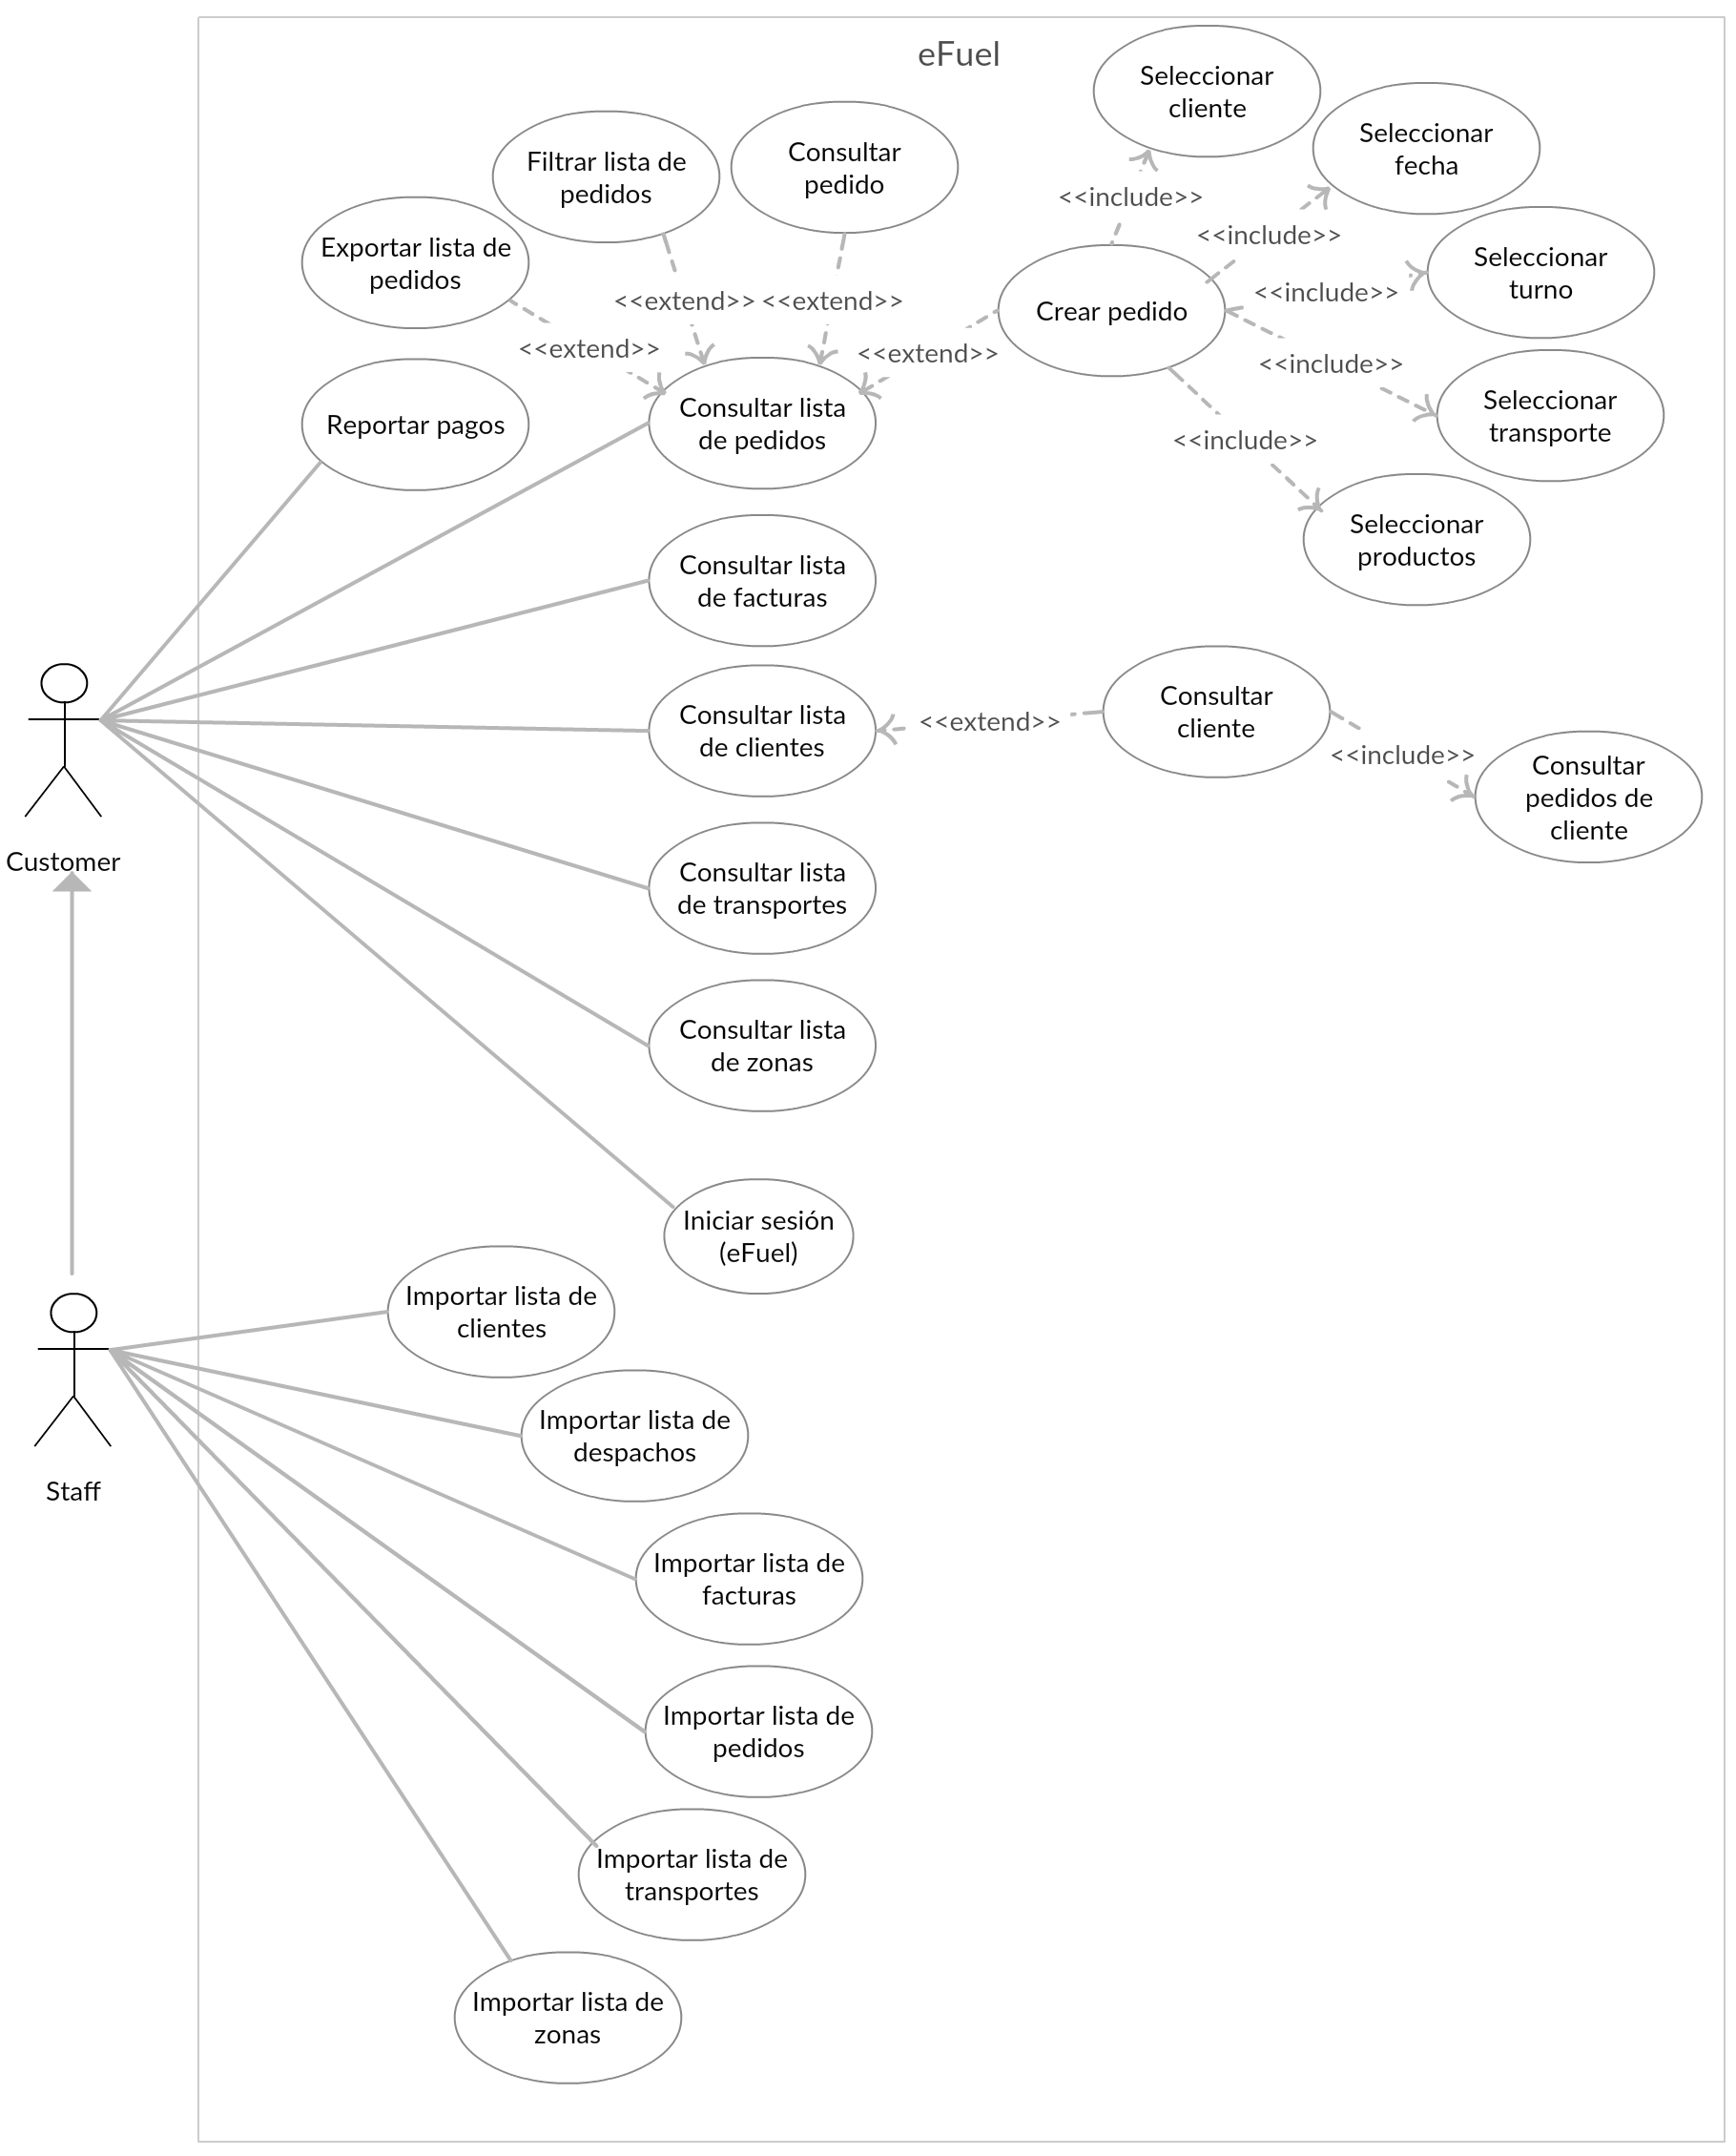
\includegraphics[width=\textwidth]{cu_customer_staff.png}
        \centering
    \end{figure}

    \subsection{Especificaciones de Casos de Uso}
    A continuación las narrativas de los casos de uso:

    \begin{center}
        \begin{longtabu} to 0.9\textwidth { | X[p] | X[p] | }
            \hline
            \multicolumn{2}{|l|}{
                \cellcolor{gray!30}{\large{\textbf{Caso de Uso:}} Gestionar usuarios}
            } \TBstrut \\
            \hline\hline

            \multicolumn{2}{|l|}{
                \makecell{\large{\textbf{Descripción:}} \\ Muestra en pantalla el módulo de gestión de miembros.}
            } \\
            \hline

            \multicolumn{2}{|l|}{
                \makecell{\large{\textbf{Precondición:}} \\ Haber ingresado la dirección correcta del sitio en la barra de navegación.}
            } \\
            \hline

            
            \multicolumn{2}{|l|}{\cellcolor{gray!15}\large{\textbf{Flujo básico:}}}  \TBstrut\\
            \hline

            Actor & Sistema \TBstrut\\
            \hline

            1. El actor abre su navegador e introduce la dirección correspondiente al back end de Umbraco. &  \\
            \hline
             & 2. El servidor procesa la solicitud y envía al navegador del cliente una ventana para que el usuario se autentique. \\
             \hline\hline


            \multicolumn{2}{|l|}{\cellcolor{gray!15}\large{\textbf{Flujos alternos:}}}  \TBstrut\\
            \hline
            Actor & Sistema \TBstrut\\
            \hline
            1. El actor hace algo. &  \TBstrut\\
            \hline
             & 2. El sistema responde. \TBstrut\\
             \hline\hline

            \multicolumn{2}{|l|}{
                \makecell{\large{\textbf{Poscondición:}} \\ Aquí va la poscondición del caso de uso}
            } \\
            \hline
            \multicolumn{2}{|l|}{
                \makecell{\large{\textbf{Requerimientos especiales:}} \\ Aquí van los requerimientos especiales del caso de uso}
            } \\
            \hline
            \multicolumn{2}{|l|}{
                \makecell{\large{\textbf{Puntos de extensión:}} \\ Aquí van los puntos de extensión del caso de uso}
            } \\
            \hline
        \end{longtabu}
    \end{center}

    \begin{center}
        \begin{longtabu} to 0.9\textwidth { | X[p] | X[p] | }
            \hline
            \multicolumn{2}{|l|}{
                \cellcolor{gray!30}{\large{\textbf{Caso de Uso:}} Consultar lista de usuarios}
            } \TBstrut \\
            \hline\hline

            \multicolumn{2}{|l|}{
                \makecell{\large{\textbf{Descripción:}} \\ Muestra en pantalla una lista con todos los miembros del sistema.}
            } \\
            \hline

            \multicolumn{2}{|l|}{
                \makecell{\large{\textbf{Precondición:}} \\ Haber ingresado exitosamente al back end de Umbraco.}
            } \\
            \hline

            
            \multicolumn{2}{|l|}{\cellcolor{gray!15}\large{\textbf{Flujo básico:}}}  \TBstrut\\
            \hline

            Actor & Sistema \TBstrut\\
            \hline

            1. El actor hace click en la pestaña de \emph{Members} en el back end de Umbraco. & \\
            \hline
             & 2. El sistema muestra una vista con la lista de los miembros. \\
             \hline\hline


            \multicolumn{2}{|l|}{\cellcolor{gray!15}\large{\textbf{Flujos alternos:}}}  \TBstrut\\
            \hline
            Actor & Sistema \TBstrut\\
            \hline
            1. El actor hace algo. &  \TBstrut\\
            \hline
             & 2. El sistema responde. \TBstrut\\
             \hline\hline

            \multicolumn{2}{|l|}{
                \makecell{\large{\textbf{Poscondición:}} \\ Aquí va la poscondición del caso de uso}
            } \\
            \hline
            \multicolumn{2}{|l|}{
                \makecell{\large{\textbf{Requerimientos especiales:}} \\ Aquí van los requerimientos especiales del caso de uso}
            } \\
            \hline
            \multicolumn{2}{|l|}{
                \makecell{\large{\textbf{Puntos de extensión:}} \\ Aquí van los puntos de extensión del caso de uso}
            } \\
            \hline
        \end{longtabu}
    \end{center}




    \section{Vista Lógica} \label{vistaLogica}
    \subsection{Vista General}
    \subsubsection{Diagrama Conceptual (Modelo de Dominio)}
    \subsubsection{Diagrama de Clases}
    \section{Vista de Implantación} \label{vistaImplantacion}

\subsection{Configuración Estándar}
\subsection{Diagrama de Despliegue}
    \section{Vista de Implementación} \label{vistaImplementacion}
    \subsection{Vista General}
    \subsection{Diagrama de Componentes}
    \section{Vista de Datos} \label{vistaDatos}
    \subsection{Diagrama de Entidad Relación (ER)}
    \subsection{Diccionario de Datos}
    \section{Componentes de Umbraco} \label{componentesUmbraco}
En esta sección se muestran los componentes desarrollados para la parte Umbraco del sistema.

\subsection{Vistas del sistema}
A continuación una lista de las vistas organizadas por carpetas. Hay una carpeta para cada \verb|SurfaceController| (ver figura \ref{fig:EF_Core_class_diagram_controllers}) además de una carpeta (\verb|Shared|) que contiene las vistas usadas por uno o más controladores (en su mayoría son Partial Views). Cada carpeta puede considerarse como el Modelo al que están asociadas cada una de las vistas dentro de ella, por esta razón nombraremos la primera columna "Modelos" ya que ayuda a entender la estructura del sistema desde el punto de vista de MVC.

\begin{longtable}{ | p{5.5em} | p{7em} | p{15em} | c | }
    \hline
    \rowcolor{gray!30}
    \multicolumn{1}{|c|}{Modelo} &
    \multicolumn{1}{|c|}{Nombre} &
    \multicolumn{1}{|c|}{Descripción} &
    \multicolumn{1}{|c|}{Partial View} \\
    \hhline{====}
    \endhead

    \hline
    \endfoot

    \endlastfoot

    Customer
        & Dashboard & Panel con las acciones principales que se pueden realizar sobre los clientes & - \\
    \cline{2-4}
        & Details & Información detallada de un cliente & - \\
    \cline{2-4}
        & Edit & Formulario para editar la información de un cliente & \checkmark \\
    \cline{2-4}
        & List & Tabla con todos los clientes que puede ver el usuario & \checkmark \\
    \hline

    Home
        & Dashboard & Mensaje de bienvenida (eventualmente debe mostrar las opciones más importantes del sistema) & - \\
    \hline

    Invoice
        & Dashboard & Panel con las acciones principales que se pueden realizar sobre las facturas & - \\
    \cline{2-4}
        & List & Tabla con las facturas & \checkmark \\
    \hline

    Membership
        & Index & Página de inicio de sesión & - \\
    \hline

    Order
        & Create & Formulario para crear un nuevo pedido & \checkmark \\
    \cline{2-4}
        & Dashboard & Panel con las acciones principales que se pueden realizar sobre los pedidos & - \\
    \cline{2-4}
        & Details & Información detallada de un pedido & - \\
    \cline{2-4}
        & List & Tabla con todos los pedidos que puede ver el usuario junto con los filtros y opciones de exportar la lista, crear un nuevo pedido y filtrar la lista de pedidos & \checkmark \\
    \hline

    Shared
        & AppTitle & Título de la página actual & \checkmark \\
    \cline{2-4}
        & Breadcrumbs & Cadena de enlaces a las páginas superiores a la página actual & \checkmark \\
    \cline{2-4}
        & LoginForm & Formulario de inicio de sesión & \checkmark \\
    \cline{2-4}
        & LogoutButton & Botón de cerrar sesión & \checkmark \\
    \cline{2-4}
        & Master & Estructura del sitio que es común a todas las páginas del sitio (excepto la página de inicio de sesión). Barra de navegación, barra lateral, título, etc. & - \\
    \cline{2-4}
        & Navbar & Barra de navegación superior & \checkmark \\
    \cline{2-4}
        & Sidebar & Barra de navegación lateral, contiene las secciones del sitio & \checkmark \\
    \hline

    Transport
        & Dashboard & Panel con las acciones principales que se pueden realizar sobre los transportes & - \\
    \cline{2-4}
        & Details & Información detallada de un transporte & - \\
    \cline{2-4}
        & Import & Formulario para importar una lista transportes & \checkmark \\
    \cline{2-4}
        & List & Tabla con los transportes que puede ver el usuario & \checkmark \\
    \hline

    Zone
        & Dashboard & Panel con las acciones principales que se pueden realizar sobre las zonas & - \\
    \cline{2-4}
        & Import & Formulario para importar una lista zonas & \checkmark \\
    \cline{2-4}
        & List & Tabla con las zonas que puede ver el usuario & \checkmark \\
    \hline

    \caption{Vistas del front end}
    \label{table:vistas}
\end{longtable}

\subsection{Doctypes y Datatypes}
\subsubsection{Datatypes}

\begin{longtable}{  l | l  }
    \hline\hline
    \rowcolor{gray!30}
    \textbf{Datatype} & \textbf{Uso} \\
    \hline\hline
    \endhead

    \hline
    \endfoot

    \endlastfoot

    Collect picker & Seleccionar un cobro \\
    Customer picker & Seleccionar un cliente \\
    Invoice picker & Seleccionar una factura \\
    Order picker & Seleccionar un pedido \\
    Product picker & Seleccionar un producto \\
    Shift picker & Seleccionar un turno \\
    Tank picker & Seleccionar un tanque \\
    Transport picker & Seleccionar un transporte del árbol de contenido \\
    Customer node picker & Seleccionar el nodo de un cliente del árbol de contenido \\
    Zone node picker & Seleccionar el nodo de una zona del árbol de contenido \\
    Attached images & Seleccionar una imagen \\
    Customer status & Elegir uno de los estados del cliente \\
    EAN-UPC & Introducir el código EAN o UPC de un producto \\
    Email address & Introducir un correo electrónico \\
    On Off & Elegir uno de 2 estados: on u off \\
    Payment terms & ELegir una forma de pago \\
    Tank list & Agregar o eliminar tanques a un transporte \\
    Textstring max65 & Introducir texto de máximo 65 caracteres \\
    Transport status & Seleccionar el estado de un transporte \\

    \hline

    \caption{Datatypes}
    \label{table:datatypes}
\end{longtable}

Todos los Datatypes creados para eFuel tienen el prefijo \emph{\_eFuel::} en su nombre.

\subsubsection{Doctypes}
El árbol de contenidos de eFuel se muestra en la figura \ref{fig:content_tree}. Luego se describen los Doctypes de la aplicación.

\begin{figure}[h]
    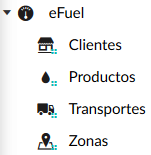
\includegraphics[width=0.3\textwidth, center]{content_tree.png}
    \caption{Árbol de contenido de eFuel}
    \label{fig:content_tree}
    \centering
\end{figure}

\begin{longtable}{ | p{5em} | l | l | }
    \hline
    \rowcolor{gray!30}
    \multicolumn{1}{|c|}{Doctype} &
    \multicolumn{1}{|c|}{Propiedades} &
    \multicolumn{1}{|c|}{Datatype} \\
    \hline
    \endhead

    \hline
    \endfoot

    \endlastfoot

    Cliente
        & Descripción & Textarea \\
        \cline{2-3}
        & Código de impuestos & Textstring \\
        \cline{2-3}
        & Estado & Customer status \\
        \cline{2-3}
        & Zona & Zone node picker \\
        \cline{2-3}
        & Forma de pago & Payment terms \\
        \cline{2-3}
        & Ok days & Numeric \\
        \cline{2-3}
        & Due days & Numeric \\
        \cline{2-3}
        & Dirección & Textstring \\
        \cline{2-3}
        & Teléfono & Textstring \\
        \cline{2-3}
        & Correo & Email address \\
        \cline{2-3}
        & Contacto & Textstring \\
        \cline{2-3}
        & Código ERP & Textstring \\
        \cline{2-3}
        & Código externo & Textstring \\
        \cline{2-3}
        & Imagen & Attached images \\
    \hline

    Producto
        & Precio base & Decimal \\
        \cline{2-3}
        & Descripción & Textarea \\
        \cline{2-3}
        & Código ERP & Textstring \\
        \cline{2-3}
        & Código externo & Textstring \\
        \cline{2-3}
        & SKU & Textstring \\
        \cline{2-3}
        & EAN/UPC & EAN-UPC \\
        \cline{2-3}
        & Imagen & Attached images \\
    \hline

    Tanque
        & Volumen & Numeric \\
    \hline

    Transporte
        & Placa chuto & Textstring \\
        \cline{2-3}
        & Placa cisterna & Textstring \\
        \cline{2-3}
        & Zona & Zone node picker \\
        \cline{2-3}
        & Nombre del conductor & Textstring \\
        \cline{2-3}
        & Volumen total & Numeric \\
        \cline{2-3}
        & Estado & Transport status \\
        \cline{2-3}
        & Tanques & Tank list \\
        \cline{2-3}
        & Código ERP & Textstring \\
        \cline{2-3}
        & Código externo & Textstring \\
        \cline{2-3}
        & Imagen & Attached images \\
    \hline

    Turno
        & Descripción & Textstring \\
        \cline{2-3}
        & Código ERP & Textstring \\
        \cline{2-3}
        & Código externo & Textstring \\
    \hline

    Zona
        & Código ERP & Textstring \\
        \cline{2-3}
        & Código externo & Textstring \\
    \hline

    \caption{Doctypes}
    \label{table:doctypes}
\end{longtable}
\end{document}

